% =====================================================================
% 𓂀 CODEX–DGM H7 COHERENCE AGENT SYSTEM v1.4
% =====================================================================
% SHADOW HEADER (CODEX STYLE / README)
%
% Project Name:
%   Codex–DGM H7 Coherence Agent System
%
% One-Line Description:
%   A coherence-gated, multi-agent architecture that constrains recursive
%   self-improvement in Darwin Gödel Machine (DGM)-style systems using the
%   Codex H7 / ΔΦ coherence horizon.
%
% Core Principle (Codex Law):
%   Recursive self-modification is permitted only when internal dynamics
%   remain coherent under bounded phase drift.
%
%   ΔΦ  → local drift (phase / instability estimator)
%   C   = 1 / (1 + |ΔΦ|)   (local coherence)
%   H7  = mean(C ≥ 0.70)  (coherence horizon)
%
%   H7 acts as:
%     • Fitness regularizer
%     • Archive admission gate
%     • Self-modification safety verifier
%
% Authorship & Credit:
%   • James Paul Jackson
%       – Originator of the Codex H7 Coherence Engine
%       – ΔΦ-based coherence framework and coherence-horizon gating
%       – Codex architecture and stability-first safety framing
%
%   • Keith L. Beaudoin
%       – Integration of H7 into DGM / EvoDistill-style evolving codebases
%       – Fitness augmentation, archive gating, and verification strategies
%
% Lineage & Inspiration:
%   • Jürgen Schmidhuber — Gödel Machine & self-referential learning systems
%   • Quality-Diversity & open-ended evolution literature
%
% Source Integration:
%   Synthesizes and formalizes ideas from:
%     Keith L. Beaudoin,
%     "Integrating H7 Engine Code into DGM Evolving Codebase", Dec 25, 2025
%
% Intended Use:
%   • arXiv / workshop submission
%   • Open-source reference implementation
%   • Safe self-improving agent systems
%
% Scope Discipline:
%   This work defines a computational stability governor.
%   It does NOT claim new physics, metaphysics, or consciousness theory.
% =====================================================================

\documentclass[11pt]{article}
\usepackage[margin=1in]{geometry}
\usepackage{amsmath, amssymb}
\usepackage{hyperref}
\usepackage{enumitem}
\usepackage{xcolor}
\usepackage{listings}
\usepackage{tikz}
\usetikzlibrary{shapes.geometric, arrows.meta, chains, positioning}

\lstset{
  basicstyle=\small\ttfamily,
  keywordstyle=\color{blue},
  commentstyle=\color{gray},
  frame=single,
  breaklines=true,
  showstringspaces=false
}

\hypersetup{
  colorlinks=true,
  linkcolor=blue,
  citecolor=blue,
  urlcolor=blue
}

\title{Coherence-Gated Darwin Gödel Agents:\\
A Codex H7 / $\Delta \Phi$ Stability Governor for Recursive Self-Improvement}
\author{
James Paul Jackson \and Keith L.\ Beaudoin
}
\date{December 2025}

\begin{document}
\maketitle

\begin{abstract}
Recursive self-improvement systems often fail due to internal drift, unstable
mutations, and archive collapse. We present a coherence-gated agent architecture
that integrates the Codex H7 / $\Delta \Phi$ coherence engine as a stability
governor inside a Darwin Gödel Machine (DGM)-style evolutionary loop.
Local coherence is computed from phase drift $\Delta \Phi$, and the H7 horizon
measures the fraction of internal states with coherence $C \ge 0.70$.
H7 is operationalized in three roles: (i) auxiliary fitness objective,
(ii) quality-diversity archive admission gate, and (iii) post-mutation
verification for self-modification. The result is a modular, interpretable,
and implementation-ready pathway for safe recursive improvement compatible
with EvoDistill and EvoDGM-style systems.
\end{abstract}

% ---------------------------------------------------------------------

\section{Introduction}
Darwin Gödel Machine (DGM)-style systems seek open-ended improvement through
recursive proposal, evaluation, and selection of self-modifications.
In practice, such systems destabilize: small internal changes can yield
disproportionate behavioral drift, reward hacking, or irreversible degradation.
This work introduces a coherence-first control layer based on the Codex H7
engine, constraining self-improvement by an internal stability horizon.

% ---------------------------------------------------------------------

\section{Codex Coherence Definitions}
Let $\Delta \Phi$ denote a local drift estimator over an internal trajectory
(e.g., activations, embeddings, gradients, or telemetry vectors). Define:
\begin{equation}
C = \frac{1}{1 + |\Delta \Phi|},
\end{equation}
and the H7 coherence horizon:
\begin{equation}
\mathrm{H7} = \mathbb{E}\left[\mathbf{1}_{C \ge 0.70}\right].
\end{equation}

\paragraph{Threshold provenance.}
The $0.70$ threshold arises empirically from repeated Codex system runs across
multiple domains, where coherence plateaus consistently emerged near
$C \approx 0.7$ as a boundary separating stable refinement from runaway drift.
It is treated here as a practical default rather than a universal constant.

\subsection{Concrete $\Delta \Phi$ Estimators}
Implementable estimators include:
\begin{itemize}[leftmargin=1.2em]
\item \textbf{Neural activations:} $\Delta \Phi_t = \|a_{t+1} - a_t\|_2$
\item \textbf{Gradient flow:} $\Delta \Phi_t = \|\nabla L_t - \nabla L_{t-1}\|$
\item \textbf{Embedding phase drift:} $\Delta \Phi_t = \arccos(\cos\_sim(e_t, e_{t+1}))$
\item \textbf{Hyperparameters / patches:} finite differences on scalar or vector series
\end{itemize}

% ---------------------------------------------------------------------

\section{H7-Gated Multi-Agent Architecture}

\begin{figure}[ht]
\centering
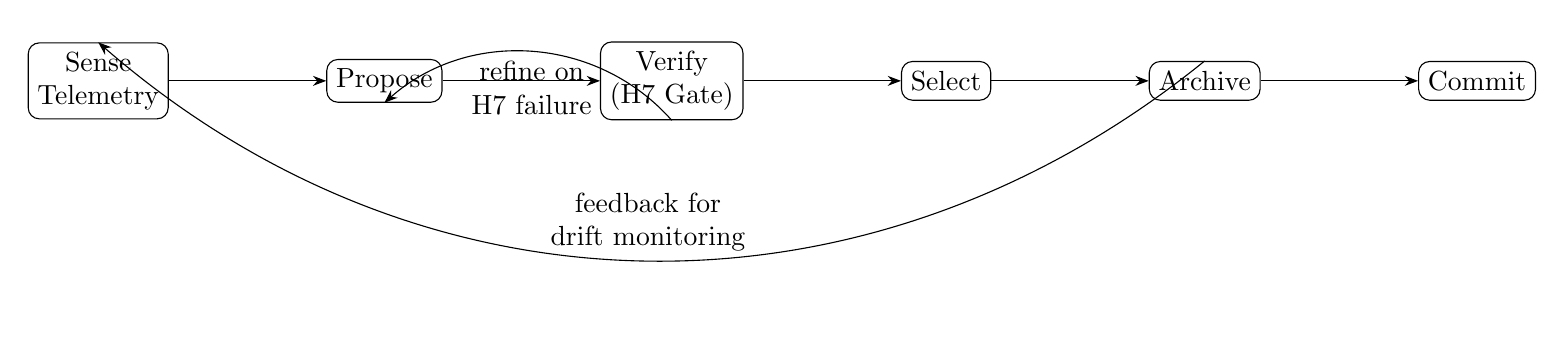
\begin{tikzpicture}[
    node distance=1.8cm and 2cm,
    start chain=going right,
    box/.style={
        rectangle,
        draw,
        rounded corners,
        minimum height=1.4em,
        minimum width=3.0em,
        align=center,
        on chain
    }
]
  \node[box] (sense) {Sense\\Telemetry};
  \node[box] (propose) {Propose};
  \node[box] (verify) {Verify\\(H7 Gate)};
  \node[box] (select) {Select};
  \node[box] (archive) {Archive};
  \node[box] (commit) {Commit};

  \draw[->, >=Stealth] (sense) -- (propose);
  \draw[->, >=Stealth] (propose) -- (verify);
  \draw[->, >=Stealth] (verify) -- (select);
  \draw[->, >=Stealth] (select) -- (archive);
  \draw[->, >=Stealth] (archive) -- (commit);

  \draw[->, >=Stealth]
    (verify.south)
    to[bend right=45]
    node[below, align=center] {refine on\\H7 failure}
    (propose.south);

  \draw[->, >=Stealth]
    (archive.north)
    to[bend left=40]
    node[above, align=center] {feedback for\\drift monitoring}
    (sense.north);
\end{tikzpicture}
\caption{H7-gated multi-agent loop with coherence-triggered refinement and archive feedback.}
\label{fig:h7_loop}
\end{figure}

\subsection{Agent Roles}
\begin{itemize}[leftmargin=1.2em]
\item \textbf{Telemetry Agent}: extracts internal trajectories and computes $(\Delta \Phi, C, \mathrm{H7})$
\item \textbf{Proposer Agent}: generates candidate self-modifications
\item \textbf{Verifier Agent}: enforces H7 coherence thresholds
\item \textbf{Archivist Agent}: maintains a coherence-gated quality-diversity archive
\item \textbf{Selector Agent}: ranks candidates via task performance and H7
\end{itemize}

% ---------------------------------------------------------------------

\section{Three Integration Points}

\subsection{Fitness Augmentation}
\begin{equation}
F(m) = \alpha Q(m) + (1-\alpha)\mathrm{H7}(m),
\end{equation}
where $Q(m)$ is task performance and $\alpha \in [0,1]$.

\subsection{Archive Admission Gate}
Candidates are archived only if:
\[
\mathrm{mean}(C) \ge 0.70 \quad \land \quad \Delta \Phi\ \text{novelty exceeds threshold}.
\]

\subsection{Self-Modification Verification}
Self-modifications are accepted only when:
\[
\mathrm{H7}(m) \ge 0.70,
\]
otherwise they are rejected or refined.

\paragraph{Compatibility note.}
H7 gating is designed to complement, not replace, other safeguards such as
minimum task-performance floors, novelty search objectives, or behavioral
diversity descriptors commonly used in quality-diversity frameworks.

% ---------------------------------------------------------------------

\section{Threshold Tuning}
The $0.70$ threshold may be tuned per domain.
Ablation sweeps over $\alpha \in \{0.5, 0.7, 0.9\}$ and $\tau \in [0.65, 0.75]$
allow calibration without destabilizing recursion.

% ---------------------------------------------------------------------

\section{Pseudocode Snippets}

\begin{lstlisting}[language=Python, caption={Core ΔΦ and H7 computation}]
def compute_delta_phi(sequence):
    diffs = sequence[1:] - sequence[:-1]
    return np.linalg.norm(diffs, axis=-1)

def compute_coherence(delta_phi):
    return 1.0 / (1.0 + abs(delta_phi))

def compute_h7(coherence, threshold=0.70):
    return (coherence >= threshold).mean()
\end{lstlisting}

\begin{lstlisting}[language=Python, caption={Verifier agent gate}]
class VerifierAgent:
    def verify(self, telemetry):
        dphi = compute_delta_phi(telemetry)
        C = compute_coherence(dphi)
        H7 = compute_h7(C)
        return H7 >= 0.70
\end{lstlisting}

% ---------------------------------------------------------------------

\section{Discussion}
This architecture reframes recursive self-improvement as a coherence-bounded
process. Rather than maximizing change, systems are permitted to evolve only
within stable internal regimes. This provides a practical, interpretable,
and safety-aligned mechanism for sustaining open-ended improvement without
destabilization.

% ---------------------------------------------------------------------

\section*{References}
\begin{enumerate}[leftmargin=1.2em]
\item Keith L.\ Beaudoin, \emph{Integrating H7 Engine Code into DGM Evolving Codebase}, Dec 25, 2025.
\item Jürgen Schmidhuber, Gödel Machine and self-referential learning systems.
\item Quality-Diversity and open-ended evolution literature.
\end{enumerate}

\end{document}
